Como discutido na introdução, o nexo entre cidadãos e governo é a base dos
sistemas democráticos. Dada a importância desse nexo não é surpresa que na
Ciência Política exista uma grande gama de trabalhos e abordagens que buscam
descrever, explicar e prevê-lo. A caracterização e justificativa para nosso
problema de pesquisa parte de um diálogo com a Teoria Política Formal, a ser
definida e discutida em seguida.

\section{Fundamentos da Teoria Política Formal}

Vamos definir Teoria Política Formal como: conjunto de modelos e hipóteses
teóricas explicitamente definidos que buscam representar atividades e
comportamentos relacionados à ação e escolha coletiva
\cite{oppenheimer2012principles,clarke2012model}.


\begin{comment}
Com essa definição estamos conjugando três definições: a de Teoria, a de
Política e a de Formal. O conceito de política, e em certa medida o de teoria,
pode ser considerado como ``essencialmente contestado'', isto é, é um conceito
cuja grande importância normativa faz com que haja uma disputa em relação à sua
definição e uso\cite{collier2006essentially}. Há assim um grande debate sobre a
melhor definição de política. Vamos usar a definição dada por Joe Oppenheimer,
para o qual a ``política consiste no comportamento realizado com o objetivo de
tomar decisões centralizadas para um grupo, ou para assegurar o interesse de
membros desse grupo'' \cite[p. I]{oppenheimer2012principles}\footnote{Essa
  definição é equivalente a dada por \citeonline{barber2003strong}. Para uma
  discussão mais aprofundada sobre o tema ver:
  \citeonline{warren1999political}.}.

Quanto a definição de teorias estamos seguindo perspectivas pós-positivistas de
ciência, particularmente a Visão Semântico-Pragmática de
\citeonline{clarke2012model} em que teorias são conjuntos de modelos, sistemas
caracterizados por uma definição, e hipóteses teóricas - a delimitação
da similaridade dos modelos com determinados sistemas alvo\footnote{Para uma
  discussão sobre as diferentes visões sobre o que são teorias e modelos ver
  \citeonline{sep-structure-scientific-theories}.}.

Por fim, entendemos que os modelos são formais na medida em que construídos por
meio de algum sistema formal \cite{wong2015formal}. Em Teoria Política Formal
isso significa que tendem a ser construídos usando o intermédio da lógica
formal, matemática ou computação \cite{morton1999methods}.
\end{comment}

Nosso foco na
literatura em teoria política formal é justificado pelo fato dela ser um corpo
teórico construído por meio de modelos
\textit{explícitos}\cite{epstein2008model}. Embora não seja a única forma de
construir modelos explícitos, o uso de um sistema formal é uma forma de forçar o
pesquisador a delimitar claramente qual o modelo está sendo utilizado para
representar um determinado sistema ou processo gerador de dados
\cite{morton1999methods, smaldino2017models}.

O estudo formal da ação e escolha coletiva teve como período de fundação moderno
o período entre \citeonline{black1948rationale} (marco no estudo da escolha
coletiva) e \citeonline{olson1965logic} (marco para os estudos da ação
coletiva). Contudo, \textit{insights} típicos da literatura foram discutidos
anteriormente por pensadores como Plínio, o Jovem (64-114 d.C.); Ramon Lull
(1232-1315); David Hume; e John Stuart Mill \cite{mclean2015strange,
  sep-free-rider, ordeshook1990emerging}.Embora não seja a única forma de se
modelar formalmente fenômenos políticos, modelos de escolha racional são em
larga medida os mais comuns \cite{austen1998social}. De uma forma geral, os
modelos da Teoria da Escolha Racional, em política, buscam representar fenômenos
segundo alguma variante da seguinte equação, a Equação de Plott
\cite{munger2015choosing, ostrom1986agenda}\footnote{Essa ``equação'' é
  conceitual. \(\oplus\) é usado como um operador abstrato não especificado
  \cite{ostrom1986agenda}. }:
\begin{figure}[H]
\begin{align*}
  \text{Preferences} \oplus \text{Beliefs}  \oplus  \text{Physical Possibilities} \oplus \text{Institutions} = \text{Outcomes}
\end{align*}
\end{figure}
Esses modelos podem ser divididos em duas variantes: \textit{thin} ou
\textit{thick} \cite{hechter1997sociological, green1996pathologies}. Ambos os
tipos de modelos são construídos com base nos pressupostos mínimos de um modelo
de ator racional: preferências racionais e racionalidade bayesiana
\cite{gintis2016individuality}. A diferença entre os dois é que os modelos
\textit{thin} não fazem pressupostos substantivos sobre os valores e objetivos
dos agentes. Neles os teóricos buscam modelar a combinação entre agentes e
instituições da maneira mais geral possível. Já modelos \textit{thick} adicionam
um conjunto de pressupostos extras sobre objetivos, valores, incerteza, com o
objetivo de representar fenômenos particulares como o comparecimento às urnas, a
competição partidária, a escolha de candidatos pelo eleitorado, independência
burocrática, o efeito fiscal de constituições, dentre outros
\cite{bendor2011behavioral}.

Todo modelo formal da escolha racional em política envolve os seguintes
elementos primitivos: o conjunto $N$ de agentes, o conjunto \(X\) de
alternativas possíveis, e para cada agente em \(N\) uma descrição de suas
preferências em relação às alternativas em \(X\) \cite[p.
263]{austen1998social}.

A preferência é uma relação de comparação de valor, onde dois conceitos são
fundamentais: o de melhor (preferência estrita), denotado por \(\succ\),  e o de igual
em valor (indiferença), denotado por \(\sim\).

A relação de preferência fraca \( \succeq \)pode ser definida da seguinte forma:

\begin{align*}
  \text{x} \succeq y \leftrightarrow x \succ y \text{ ou } x \sim y
\end{align*}

A aplicação dessa definição de preferência no modelo do ator racional pressupõe
que ela seja uma relação binária no conjunto de alternativas com as seguintes
propriedades: completude, transitividade e independência das alternativas
irrelevantes \footnote{Definidas no Apêndice A.} \cite{gintis2016individuality,
  binmore2008rational}. Um pressuposto adicional é que existe uma alternativa
preferida a todas as outras para cada agente, de forma que num ambiente sem
restrição os atores escolhem essa alternativa \cite{gintis2016individuality}.
Esses pressupostos constituem o primeiro princípio do modelo do ator racional:
os agentes possuem \textit{preferências consistentes ou racionais}.

Uma conveniência analítica é representar relações de preferência por meio de
funções de utilidade, que são funções que atribuem um número real para cada
elemento do conjunto de alternativas \cite{sep-preferences}. A relação \( \succeq\) é
representada pela função \(u\): \(X \longrightarrow \mathbb{R}\) se e somente se:

\begin{align*}
  u(x) \geq u(y)
  \text{ se e somente se }
  x \succeq y
\end{align*}

Por meio dessa representação podemos dizer que os atores agem \textit{como se}
estivessem maximizando sua função de utilidade. Importante notar que funções de
utilidade são um dispositivo matemático. Modelar agentes por meio de funções de
utilidade não implica que eles sejam egoístas, instrumentais, utilitários,
hedonistas, ou que estejam ``tentando maximizar sua utilidade''
\cite{gaus2007philosophy}.

O segundo princípio dos modelos de ator racional é a \textit{racionalidade
  bayesiana} \cite{gintis2016individuality}. Quando as alternativas são
probabilísticas primeiro pressupomos que os agentes têm um \textit{modelo do
  mundo} \cite{acemoglu2011opinion}: os agentes vão ter uma crença, representada
por meio de uma função de distribuição de probabilidade, a qual vai atribuir uma
probabilidade \(p\) para cada evento em \(X\). O modelo da escolha racional
então pressupõe que as crenças dos agentes são coerentes ou consistentes, o que
equivale a dizer que estão em conformidade com os axiomas da probabilidade
\cite{jackman2009bayesian}.O primeiro elemento da racionalidade bayesiana é a
consistência das crenças dos agentes com os axiomas da probabilidade. O outro
elemento do princípio da racionalidade bayesiana é a \textit{atualização
  bayesiana}: os agentes atualizam suas crenças segundo o Teorema de Bayes
\cite[p.104]{gintis2016individuality}.

Sumarizando, os modelos de escolha racional na sua versão mais básica pressupõem
agentes com preferências consistentes, o que implica que sejam transitivas,
completas e independente de alternativas irrelevantes. Caso o contexto de
decisão seja incerto também pressupõem que os agentes têm uma crença em
conformidade com os axiomas da probabilidade  e as atualizam de acordo com o
Teorema de Bayes.


\section{Teoria Política Espacial}

Dentre as várias formas de modelar política por meio do modelo do ator racional
a a principal é o conjunto de modelos conhecido como Teoria Espacial (ou
Geométrica\footnote{Vamos usar o termo geométrico de maneira intercambiável com
  espacial, pelo fato do último gerar a confusão com trabalhos relacionados ao
  papel do espaço geográfico em política \cite{ward2002spatial,
    poole2005spatial}.}) de Política \cite{van2005political}.

A Teoria Espacial de Política tem suas origens nos trabalhos canônicos de Duncan
Black e Anthony Downs, e as bases matemáticas da teoria foram desenvolvidas por
Otto Davis, Melvin Hinich e Peter Ordeshook \cite{black1958theory,
  downs1957economic, poole2005spatial, miller2015spatial}. Tal teoria está
fundamentada na idéia essencial que as alternativas, posicionamento e
preferências dos agentes políticos podem ser representadas por meio de espaços
geométricos. Captura a metáfora e noção da linguagem política diária de que a
similaridade/diferença entre alternativas, posicionamentos e preferências
políticas pode ser pensada por meio de relações de proximidade/distância, tal
qual a noção de que partidos, pessoas, ou propostas são de ``extrema-esquerda'',
``centristas'' ou ``de direita'' \cite{munger2015choosing}. Suponha que João e
Alice tenham preferências similares e que João e Eva tem preferências
divergentes. Então podemos dizer que João é mais ``próximo'' de Alice devido ao fato
dele ser mais parecido com ela do que com Eva. O espaço político é então um
espaço conceitual no qual a noção de similaridade é mapeada à de proximidade
\cite{laver2014measuring}.


Seguindo \citeonline{humphreys2010spatial}, podemos dividir os modelos
geométricos em dois grupos. Eles podem ser \textit{fracamente} ou
\textit{fortemente} espaciais. Os modelos fracamente espaciais só caracterizam
as alternativas e as preferências segundo uma analogia geométrica. Já modelos
fortemente espaciais envolvem uma teoria comportamental sobre como as pessoas
pensam sobre política \cite{laver2014measuring}.


Nos modelos fracamente espaciais o conjunto de alternativas \(X\) é pensado como
um espaço, mais comumente como o subconjunto de um espaço Euclidiano de \(n\)
dimensões \cite{austen1998social}. Assumem também que agentes tem preferências,
consistentes, sobre esse espaço. Não assume-se, contudo, que os agentes percebem
as utilidades das alternativas em termos das distâncias relativas no espaço
subjacente. Os agentes têm funções de utilidade abstratas, não especificadas
\cite{humphreys2010spatial}\footnote{\citeonline{humphreys2010spatial} indica o
  programa de pesquisa sobre o caos em decisões coletivas multidimensionais
  como exemplo de modelos fracamente espaciais.}.

Modelos fortemente espaciais, por outro lado, pressupõem que os agentes tem uma
cognição geométrica. Isso significa que localizam as alternativas e sua
alternativa preferida \(x_i\), seu ponto ideal, num espaço cognitivo, e
ranqueiam as alternativas segundo uma medida de distância \(d_i(.,.)\). A função
de utilidade dos agentes é a composição da função de distância e uma função de
perda de forma que \(u_i(y) = f_i(d_i(x_i,y)) \) \cite{humphreys2010spatial,
  laver2014measuring}.

O pressuposto mais comum é que a métrica seja Euclidiana: os agentes medem a
distância entre dois pontos no espaço de alternativas usando o Teorema de
Pitágoras \cite{munger2015choosing}. Ademais, assume-se, por conveniência
analítica, funções com um único pico ( o ponto ideal do agente) e simétricas.
Funções de utilidade usualmente utilizadas na ciência política são a linear, a
quadrática e a gaussiana, ilustradas na Figura 1:

\begin{figure}[H]
  \centering 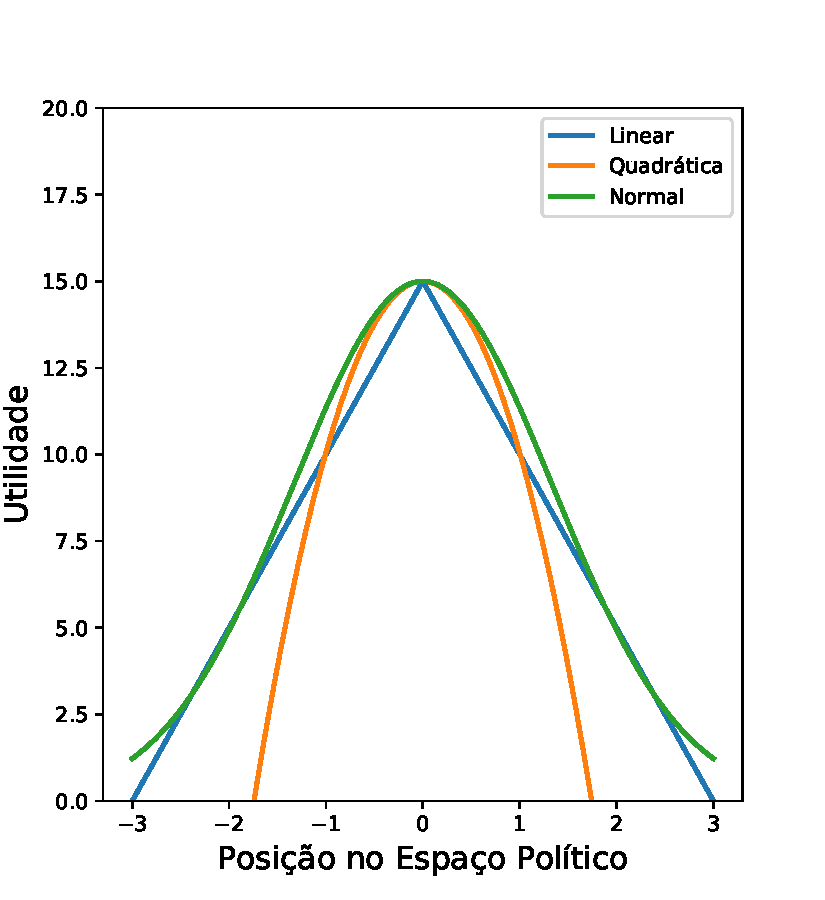
\includegraphics[scale = 0.6]{ims/utilities.pdf}
  \caption{Funções de Utilidade comuns em Política}
  \source{ Adaptado de \citeonline{armstrong2014analyzing}}
\end{figure}

Desde \citeonline{black1958theory}, essa estrutura básica do modelo espacial é
aplicada em dois tipos de fenômenos: votos em comitê e eleições de massa
\cite{munger2015choosing}. Há, contudo, uma grande diferença entre essas duas
situações de ação, e essa diferença motiva nosso problema.


\section{Teoria Espacial e Eleições}


A diferença entre os dois contextos de ação é reconhecida desde as contribuições
de Black e Downs. Em geral, em votos em comitê o número de agentes é pequeno, os
agentes são bem informados e a decisão costuma ter alta implicação para eles. Já
em eleições de massa existem muitos eleitores, a informação sobre as
alternativas é ambígua e os efeitos da decisão são, em geral, difusos
\cite{munger2015choosing}.

Essa distinção tem por corolário uma maior conformidade do voto em comitês com
os \textit{pressupostos de similaridade} entre um modelo de ator racional e uma
situação de interesse alvo. O primeiro pressuposto de similaridade refere-se a
propriedades dos agentes alvo: as crenças e preferências deles são independentes
\cite{binmore2008rational}. Os outros três lidam com o contexto de ação alvo: a
situação de ação é simples, tanto em estrutura, quanto informacionalmente; os
agentes têm incentivo para agir e informar-se; e há tempo disponível para os
agentes aprenderem \cite{binmore2007work, page2008uncertainty}. Esses
pressupostos referem-se a capacidade do analista imputar os pressupostos do
modelo do ator racional a grupos de agentes em determinadas situações. Usar o
modelo do ator racional não tem por implicação acreditar que os agentes agem
racionalmente em toda situação, mas somente que podemos justificar as
simplificações do modelo na situação de interesse da análise.

A aplicação do modelo racional ao contexto do comportamento eleitoral é assim
não trivial, por uma razão: a escala. Como argumenta \citeonline{binmore2008rational}
a aplicação do modelo da decisão racional em  ``large worlds'' é problemática,
pois provavelmente estaremos violando algum dos pressupostos de similaridade
apresentados.

Desde seu surgimento o programa de pesquisa ``Downsiano'' reconhece a distância
entre a aplicação ideal, do ponto de vista preditivo, e o sistema alvo,
eleições. \citeonline{downs1999teoria} dedica uma grande porção do livro à
incerteza e a problemas de incentivos, e a obra inspirou uma ampla literatura
sobre comparecimento às eleições, tomada de decisão do eleitor e competição
partidária \cite{bendor2011behavioral}.

Em relação à tomada de decisão do eleitor há uma tensão entre a literatura em
teoria formal e a literatura em psicologia política: a primeira costuma
pressupor que agentes têm ideologias bem definidas e são bem informados, ou tem
alguma noção probabilística, sobre as alternativas partidárias, algo contestado
veementemente pela segunda \cite[p.5]{bendor2011behavioral}. A falta de
conhecimento sobre temas/questões e a instabilidade dos posicionamentos dos
respondentes nos \textit{surveys} é um dos resultados recorrentes na literatura
em opinião pública  desde sua fundação \cite{berelson1952democratic,
  converse2006nature, zaller1992simple, kuklinski2000misinformation}.

A instabilidade nas respostas e a suscetibilidade dos cidadãos a \textit{framing
  effects}\footnote{\textit{Framing effects} são ``situações nas quais formas
  alternativas de apresentar uma questão política levam a diferentes respostas
  do público'' \cite[p.56]{bartels2003democracy}.} levam
\citeonline{bartels2003democracy} a contestar o uso da noção de preferência como
base para o estudo do nexo democrático, pois cidadãos não teriam preferências
consistentes, coerentes ou estáveis. Ele argumenta, contudo, que os eleitores
têm posicionamentos, os quais são melhor teorizados como
\textit{atitudes}\footnote{ Ele define atitude como uma tendência psicológica
  que é expressa pela avaliação de uma entidade particular com algum grau de
  aprovação ou desaprovação \cite[p.52]{bartels2003democracy}.}.

Embora possa-se contestar a validade externa dos questionários que buscam
demonstrar a instabilidade de posicionamento dos cidadãos
\cite{druckman2012public}, e a relevância dos \textit{framing effects} para a
aplicação modelo do ator racional \cite[p. 107]{gintis2016individuality},
Bartels levanta um ponto incontornável: o pressuposto de preferências racionais
não é inócuo, em especial no contexto eleitoral.

O pressuposto de que agentes têm preferências racionais sobre todas questões
políticas é exigente do ponto de vista cognitivo. Contudo, isto não é
necessário. Para aplicar o modelo geométrico de política em um contexto macro
não é necessário supor que cada questão (\textit{issue}) vá definir uma dimensão
no espaço de alternativas. O que é necessário é que os agentes tenham
\textit{algum} posicionamento nas questões, e que exista uma interrelação entre
a resposta do eleitor entre posicionamentos, de forma que possamos descrever as
atitudes dos agentes em todas as questões segundo a correlação com alguma
dimensão latente \cite{poole2005spatial,laver2014measuring}.
\citeonline{poole1985ideology} demonstram que $80\%$ dos votos no Congresso
americano podem ser explicados por uma única dimensão latente
(liberal-conservador). Já \citeonline{benoit2006party} encontra que no máximo
três dimensões são necessárias para capturar a informação relevante sobre os
posicionamentos dos eleitores, em um banco de dados de 47 países.

A preferência dos agentes nessas dimensões é, portanto, construída a partir do
posicionamento, atitudes, considerações, opiniões e crenças, deles num
agrupamento de questões. Isso significa que as preferências dos eleitores são
\textit{extrínsecas}. Preferências intrínsecas são preferências irredutíveis.
Independem de mudanças do ambiente ou de alguma razão em particular. O agente
\(i\) simplesmente prefere \(x\) a \(y\). Já preferências extrínsecas dependem
de um julgamento, uma crença, de que uma alternativa, é, em algum sentido, melhor
que a outra. Preferências extrínsecas têm razões subjacentes, e, portanto,
possivelmente mudam quando ocorrem mudanças no ambiente \cite{liu2010wright,
  binmore2008rational}.

Preferências extrínsecas violam o pressuposto de que as preferências e crenças
dos agentes são independentes, o que complica a análise da situação de ação por
meio do modelo do ator racional, dado que não podemos pressupor que elas são
estáveis. No contexto da economia do bem-estar, por exemplo,
Kenneth Binmore argumenta que os modelos do ator racional supõem
preferências intrínsecas, na medida que ``não ajudaria muito [...] introduzir uma
reforma que todos aprovam se ela mudar o ambiente de uma forma que reverta as
preferências de todos '' \cite[p.6]{binmore2008rational}.

Como as preferências no contexto macro necessariamente são construídas a partir
de posicionamentos num conjunto de questões, por definição, elas são
extrínsecas. Logo, são, potencialmente, sensíveis à mudanças no ambiente.Tendo
em vista tanto a complexidade informacional do contexto, quanto os baixos
incentivos à busca de informação, isso vai significar que os agentes serão
\textit{incertos} quanto às suas preferências. Essa incerteza em relação às
preferências, e o baixo custo, percebido, da mudança permitem que modelos de
dinâmicas de opinião possam ser usados para representar seu processo de formação
e cristalização\footnote{É claro que poderíamos usar modelos de dinâmicas de
  opinião para modelar as mudanças de crenças dos agentes. O que estamos
  afirmando é que possível utilizá-los para modelar o surgimento de
  \textit{preferências}, ou ao menos de alternativas ou pontos preferidos.}.
Convergimos assim para um argumento análogo ao da escola de Michigan de opinião
pública : o direcionamento político, ou ideologia, do agente é resultado, ou
construído, a partir de um ``campo de atitudes'' ou sistema de crenças, que no
Capítulo 4 chamaremos de perfil ideológico, o qual por sua vez é explicável por
meio da socialização do agente, a interação de suas atitudes com as atitudes dos
pares \cite{figueiredo2008decisao}. No Capítulo 3 discutimos a literatura em
dinâmicas de opinião que nós dá o arcabouço para modelar esse processo.

As preferências ideológicas dos cidadãos não são estáticas. Isso não significa,
contudo, que estas necessariamente serão altamente instáveis. Como as
preferências são construídas a partir de um conjunto de posicionamentos e
crenças em várias questões, é de se esperar que elas sejam mais estáveis do que
o posicionamento dos atores em cada questão específica
\cite{druckman2012public}. Do ponto de vista macro, é de se esperar, desta
forma, que a distribuição de preferências dos eleitores seja consistente. A
Figura 2, a qual mostra o auto-posicionamento político, numa escala de 0 a 10
(esquerda-direita), de respondentes, cuja frequência de resposta é dada no eixo
vertical, \footnote{A cada edição uma nova amostra é selecionada.} em seis
edições do \textit{European Social Survey}\footnote{Cuja página oficial é :
  \url{http://www.europeansocialsurvey.org/}}, condiz\footnote{Para questões
  metodológicas em relação a esses dados ver o Apêndice 1.} com essa
expectativa:

\begin{figure}[H]
  \centering 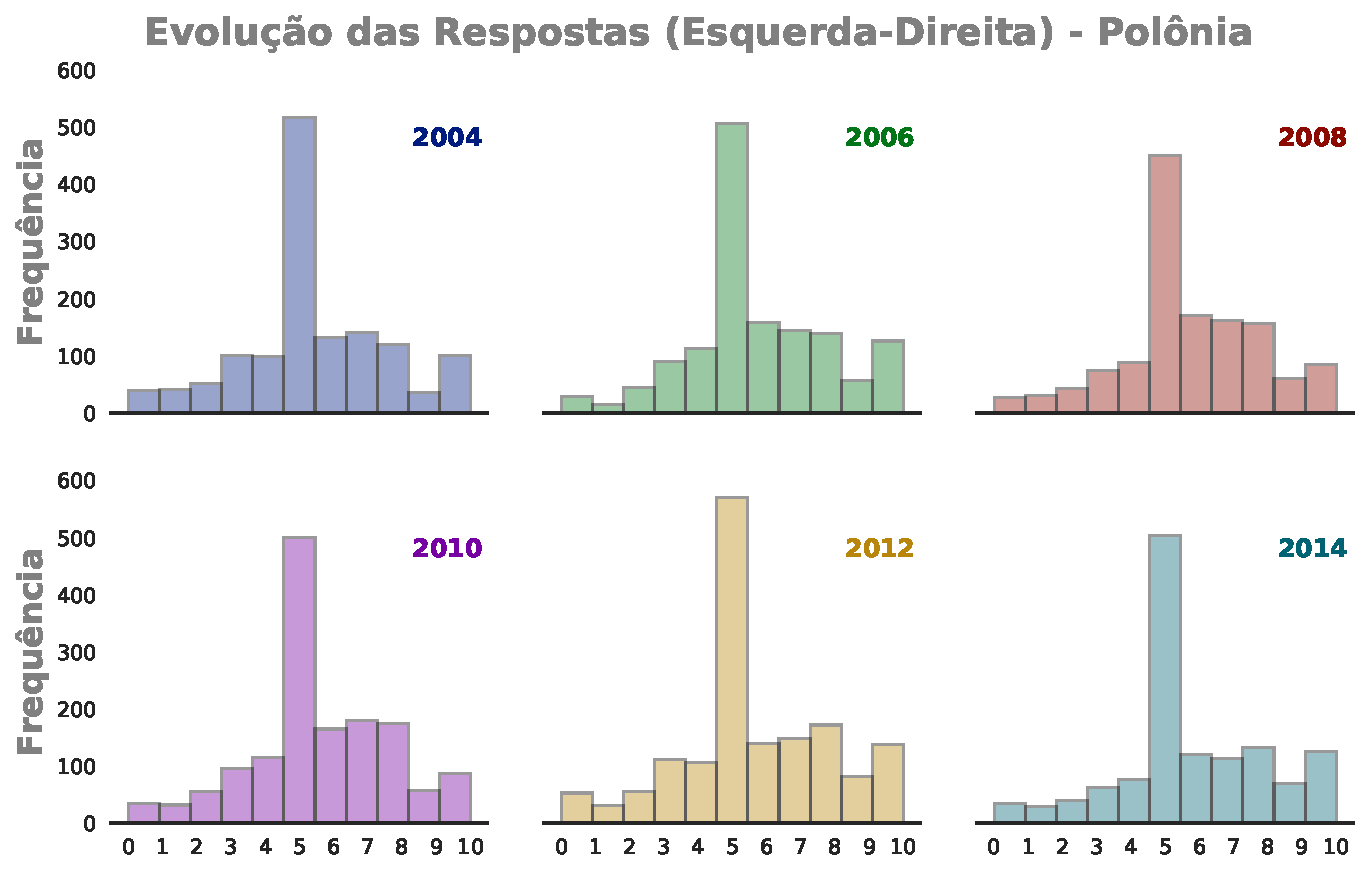
\includegraphics[width = \textwidth]{ims/ess_Pol_plots.pdf}
  \caption{Evidência de estabilidade ideológica}
  \source{O autor. Dados do \textit{European Social Survey}.}
\end{figure}

A escala do fenômeno eleitoral também afeta uma segunda categoria de agentes: os
partidos. Os partidos também estão posicionados no espaço de alternativas \(X\)e
competem pelos votos dos eleitores. Para os partidos \(X\) é um espaço de
plataformas. Para competirem têm de ser capazes de determinar qual o percentual
de votos das posições nesse espaço. A literatura reconhece que talvez os
partidos não sejam capazes de fazê-lo, adicionando a possibilidade de que eles
sejam incertos quanto as preferências políticas dos eleitores
\cite{glazer1989model, grofman2004downs}.


Como argumenta \citeonline{page2008uncertainty} essa estratégia de
modelagem consiste em ignorar a dificuldade da tomada de decisão e a
complexidade do ambiente em que os agentes estão situados, e modelá-los como
otimizadores sob incerteza. Para a competição política espacial com dimensão
$n>1$, argumenta \citeonline{laver2011party}, agir de maneira ótima é, contudo,
impossível. Isto porquê a competição política espacial é um caso particular de
modelos de tesselação dinâmica. Eles argumentam que a competição política
espacial pode ser pensado como um Jogo de Voronoi, onde \(n\) jogadores tem
\(p\) pontos para inserir num espaço n-dimensional. Cada jogador insere um ponto
em sequência buscando controlar o conjunto de regiões com o maior volume. No
caso \(n=1\) esse jogo tem solução analítica, assim como nos modelos de
competição espacial. Nos casos \(n>1\), contudo, não existe um sistema de
equaçõe que o resolva analiticamente nem há um limiar superior no tempo
necessário para resolvê-lo computacionalmente (o jogo é PSPACE-completo)
\cite[p.24]{laver2011party}.

A implicação metodológica e comportamental desse resultado é que somos levados a
modelar os partidos necessariamente agindo segundo heurísticas e se movimentando
no \textit{electoral landspace} de forma adaptativa \cite{kollman1998political,
  de1999adaptive}. Isso abre a possibilidade, teórica, de que os partidos fiquem
presos em picos locais. Do ponto de vista empírico,
\citeonline{lorenz2017modeling} e \citeonline{flache2017} apontam os seguintes
fatos estilizados sobre as distribuições de auto-posicionamento ideológico,
ilustradas na Figura 3: há um pico central dominante; há uma tendência para a
existência de \textit{clusters} não centrais, mas não extremos; e há uma
tendência a picos nos extremos.

\begin{figure}[H]
  \centering 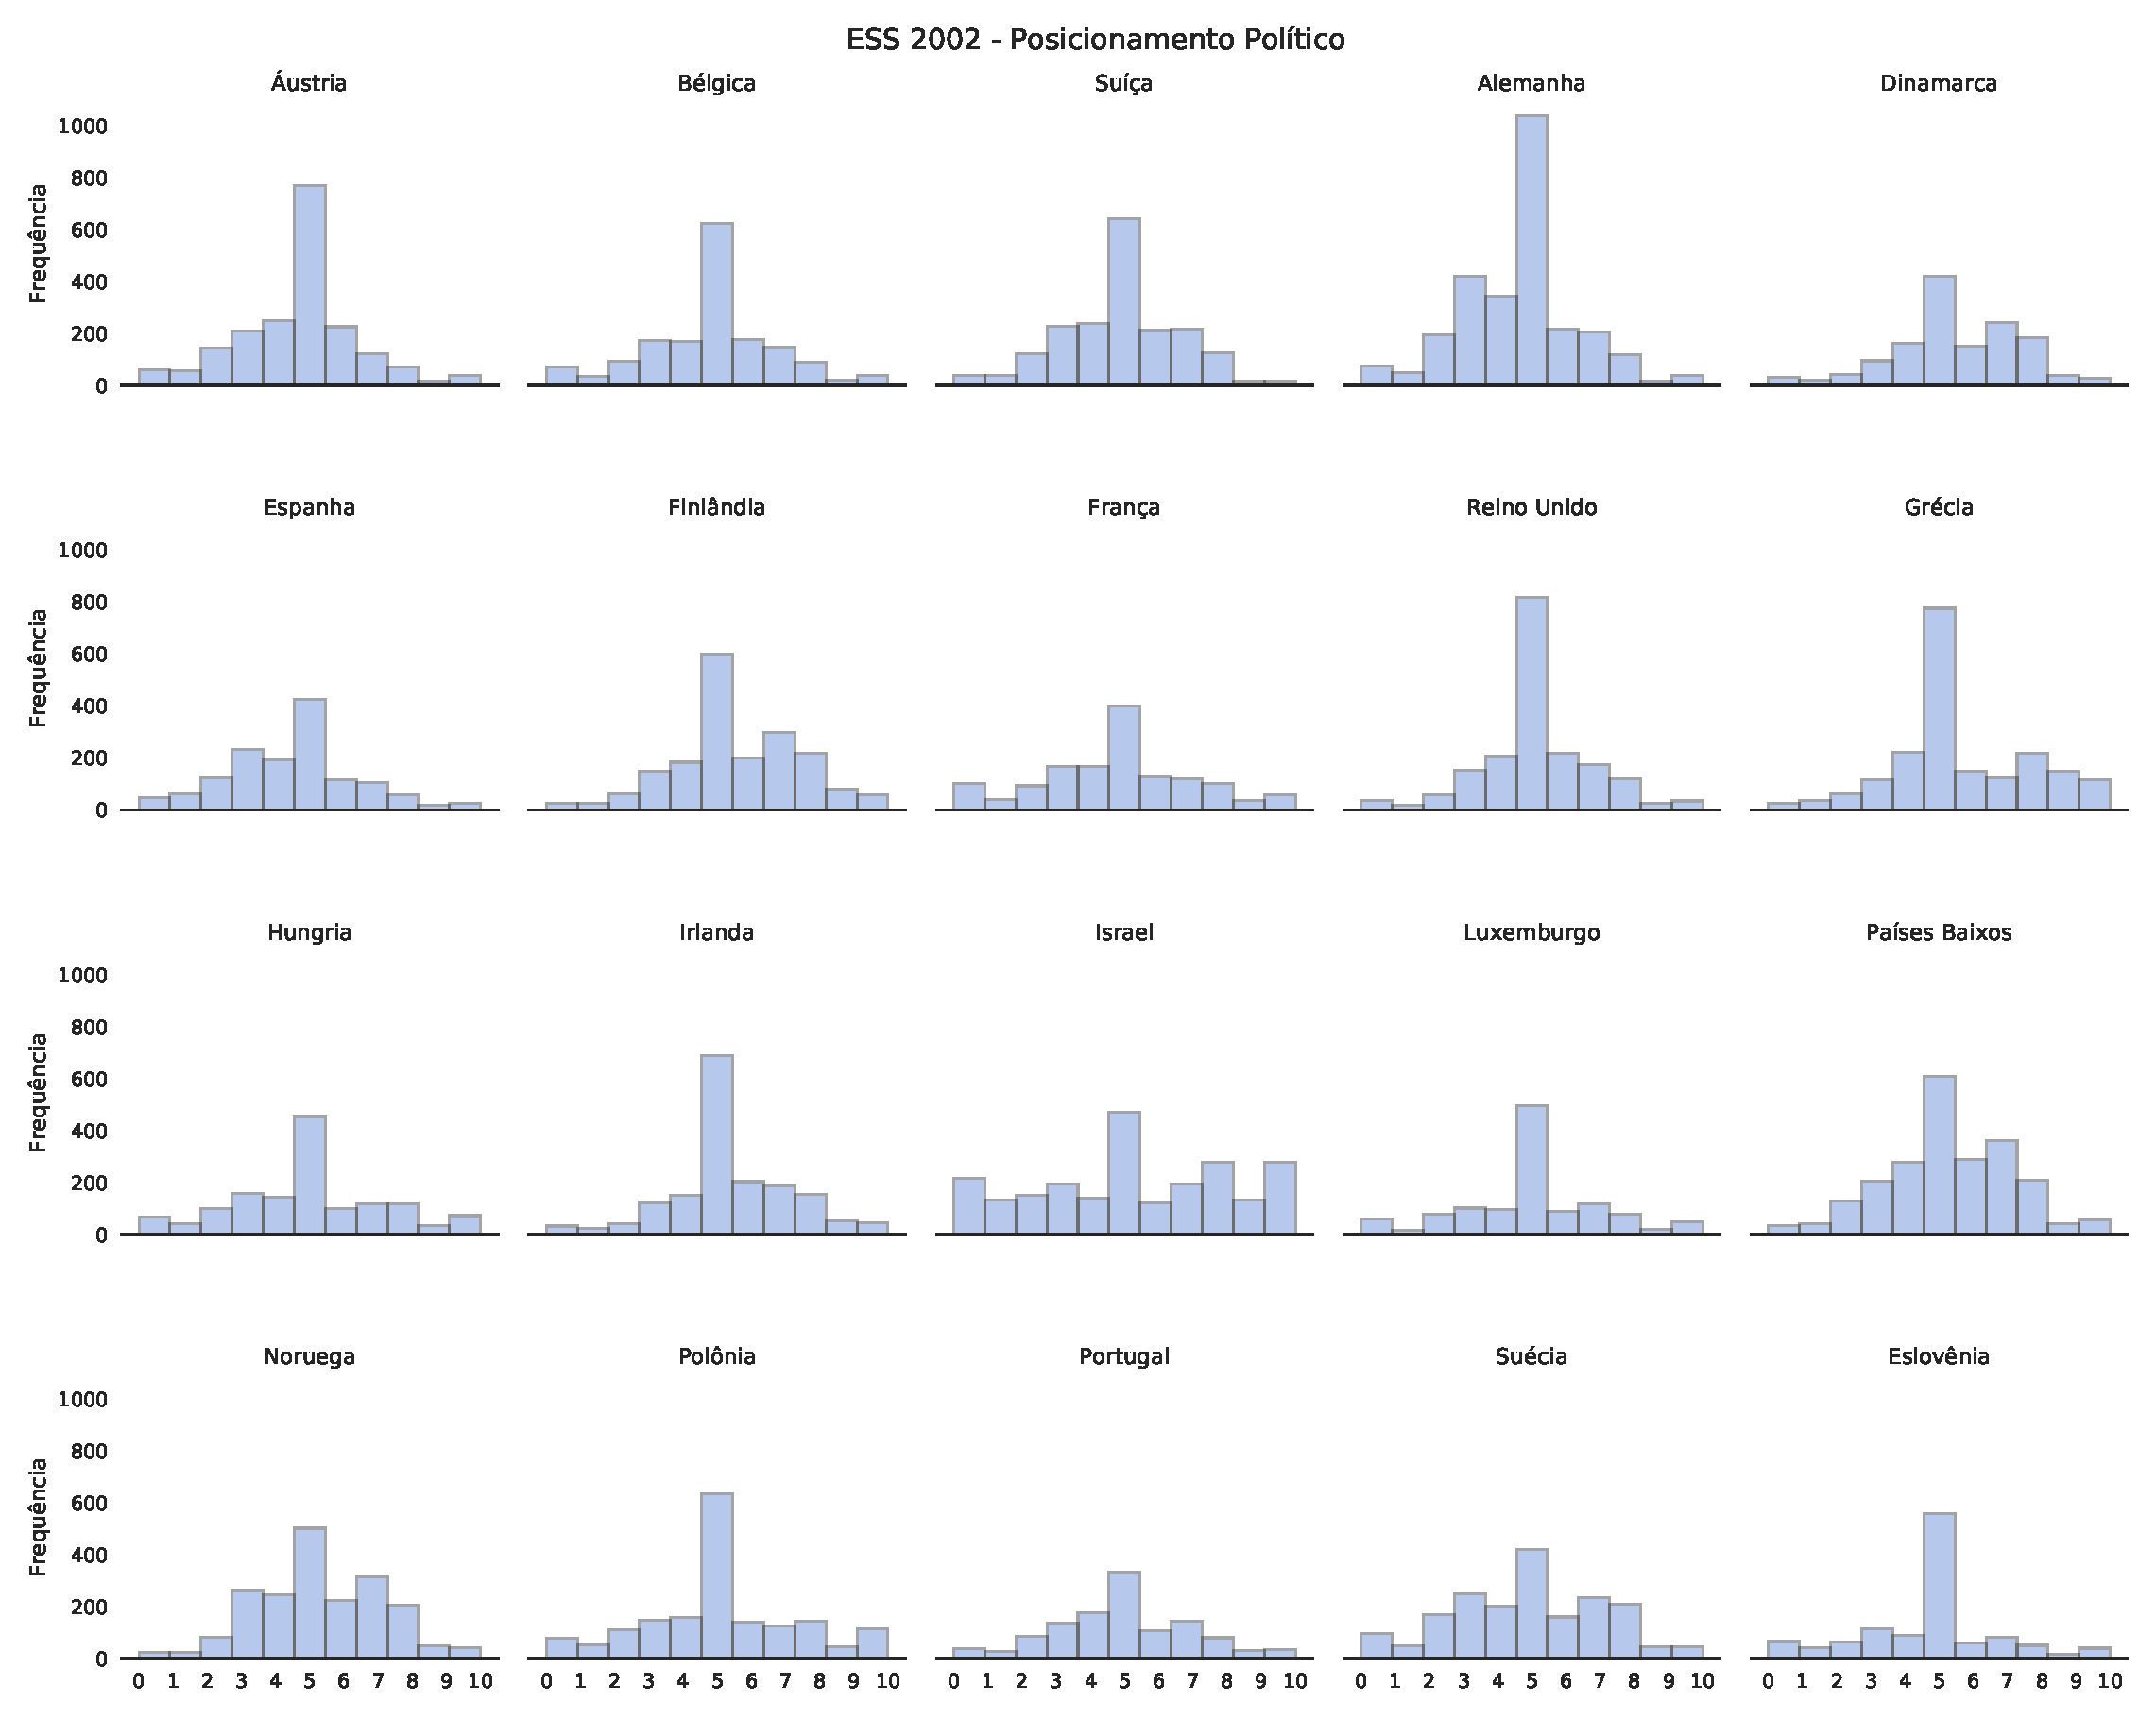
\includegraphics[width= \textwidth, height = 15cm]{ims/ess_2002_plots.pdf}
  \caption{Distribuição de Posicionamento Ideológico de respondentes em 20 países}
  \source{ O autor. Dados do \textit{European Social Survey}.}
\end{figure}

Dado que as eleições são o principal mecanismo de conexão entre cidadãos e
governo nas poliarquias \cite{dahl1989democracy} e uma vez que a sobrevivência
dos partidos na competição eleitoral depende da sua capacidade de captar o voto
dos eleitores, podemos concluir que o \textit{formato} da distribuição das
preferências dos eleitores é central para o estudo do nexo democrático.

Temos, desta forma, duas diretrizes para o estudo. Do ponto de vista micro,
podemos modelar os pontos ideais dos agentes segundo um modelo de dinâmicas de
opinião. Esse é o nosso ponto de partida. Do ponto de vista macro, aspiramos que
nossos modelos consigam gerar distribuições que sejam plausíveis do ponto de
vista empírico, dado que o formato delas importa. Esse é o nosso ponto de
referência.





%%% Local Variables:
%%% mode: latex
%%% TeX-master: "master"
%%% End:
